In the heart of Algoria, during the annual festival, a thrilling challenge called \textbf{The Great Box Shuffle} captivates all who attend. The challenge involves two long rows of enchanted boxes, each containing a collection of mystical items. The boxes in the two rows are enchanted in such a way that, with a bit of magic, their contents can be shuffled to match each other.

\begin{center}
  \def \htmlPixelsInCm {45}  % pixels in 1 centimeter in HTML mode
  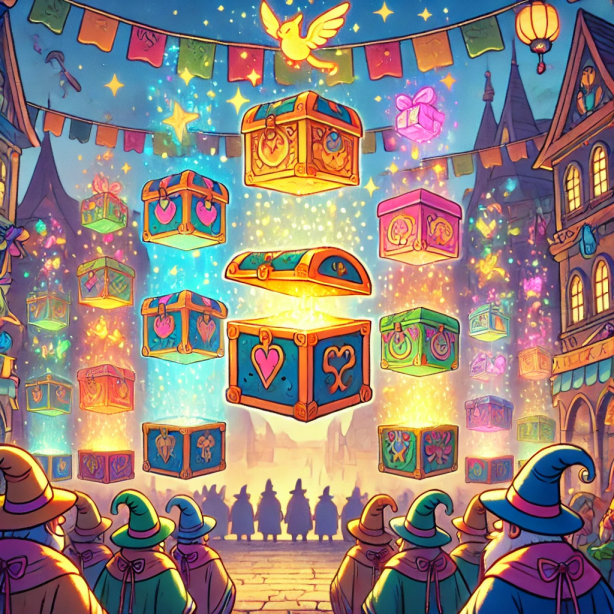
\includegraphics[width=4cm]{box.png} \\
  \small{The Great Box Shuffle festival in Algoria}
\end{center}

You are the chosen contestant this year, and your task is to determine if specific groups of boxes from the first row can be rearranged to perfectly match groups of boxes from the second row. However, the magical rules of the festival only allow you to shuffle the items within a contiguous group of boxes, rotating them either to the left or right.

Throughout the challenge, you will be given several queries. Each query will ask if a particular group of boxes from the first row can be rearranged to match a group of boxes from the second row using the allowed shuffling magic.

More formally, you are given two sequences \( A \) and \( B \), each of length \( N \). You need to answer \( q \) queries. Each query is defined by four integers \( l_1 \), \( r_1 \), \( l_2 \), and \( r_2 \). For each query, you must determine if the subarray \( A[l_1..r_1] \) can be shuffled to match the subarray \( B[l_2..r_2] \) by rotating the items within the selected segment.